\documentclass[main.tex,fontsize=8pt,paper=a4,paper=portrait,DIV=calc,]{scrartcl}
% Document
\usepackage[T1]{fontenc}
\usepackage[utf8]{inputenc}
\usepackage[dvipsnames]{xcolor}
\usepackage[nswissgerman,english]{babel} 
\usepackage{hyperref}
\renewcommand{\familydefault}{\sfdefault}

% Format
\usepackage[top=5mm,bottom=1mm,left=5mm,right=5mm]{geometry}
%\setlength{\headheight}{\baselineskip}
%\setlength{\headsep}{0mm}

%\usepackage{scrlayer-scrpage}
%\clearpairofpagestyles
%\chead{{\bfseries\TITLE, \AUTHOR, \pagename~\thepage}}

%\addtokomafont{pagehead}{\upshape}

\usepackage{multicol}
\setlength{\columnsep}{2mm}
\setlength{\columnseprule}{0.1pt}

% Math
\usepackage{amsmath}
\usepackage{amssymb}
\usepackage{amsfonts}

% Code
\usepackage{fancyvrb, etoolbox, listings, xcolor}
%\usemintedstyle{bw}

%\newminted[shell]{bash}{
%fontsize=\footnotesize,
%fontfamily=tt,
%breaklines=true,
%frame=single,
%framerule=0.1pt,
%framesep=2mm,
%tabsize=2
%}
%\newminted{css}{
%breaklines=true,
%tabsize=4,
%autogobble=true,
%escapeinside=||,
%stripall=true,
%stripnl=true,
%}

    \definecolor{lightgray}{rgb}{0.95, 0.95, 0.95}
    \definecolor{darkgray}{rgb}{0.4, 0.4, 0.4}
    \definecolor{purple}{rgb}{0.65, 0.12, 0.82}
    \definecolor{ocherCode}{rgb}{1, 0.5, 0} % #FF7F00 -> rgb(239, 169, 0)
    \definecolor{blueCode}{rgb}{0, 0, 0.93} % #0000EE -> rgb(0, 0, 238)
    \definecolor{greenCode}{rgb}{0, 0.6, 0} % #009900 -> rgb(0, 153, 0)
    \definecolor{teal}{rgb}{0.0, 0.5, 0.5}

\lstdefinestyle{code}{
    identifierstyle=\color{black},
    keywordstyle=\color{blue}\bfseries\small,
    ndkeywordstyle=\color{greenCode}\bfseries\small,
    stringstyle=\color{ocherCode}\ttfamily\small,
    commentstyle=\color{teal}\ttfamily\textit\small,
    basicstyle=\ttfamily\small,
    breakatwhitespace=false,         
    breaklines=true,                 
    captionpos=b,                    
    keepspaces=true,                 
    showspaces=false,                
    showstringspaces=false,
    showtabs=false,                  
    tabsize=2,
    belowskip=-5pt
}



% Images
\usepackage{graphicx}
\newcommand{\pic}{\includegraphics[scale=0.3]}
\graphicspath{{Screenshots/}{../Screenshots}}
\makeatletter
\def\pictext#1#2{%
    \@ifnextchar[{%
    \pictext@iiiii{#1}{#2}%
    }{%
      \pictext@iiiii{#1}{#2}[0.5,0.4,0.3]% Default is 5
    }%
}
\def\pictext@iiiii#1#2[#3,#4,#5]{\begin{minipage}{#3\textwidth}\includegraphics[scale=#4]{#1}\end{minipage}\begin{minipage}{#5\textwidth}#2\end{minipage}}
\def\minipg#1#2{%
    \@ifnextchar[{%
    \minipg@iiii{#1}{#2}%
    }{%
      \minipg@iiii{#1}{#2}[0.3,0.6]% Default is 5
    }%
}
\def\minipg@iiii#1#2[#3,#4]{\vspace{0.8mm}\begin{minipage}{#3\textwidth}#1\end{minipage}\begin{minipage}{#4\textwidth}#2\end{minipage}{\vspace{0.8mm}}}
\makeatother

%\newenvironment{minty}[2]% environment name
%{% begin code
%  \begin{minipage}{#1}
%  \begin{minted}{#2}
%}%
%{% end code
%  \end{minted}
%  \end{minipage}
%  \end{minty}\ignorespacesafterend
%} 

% Smaller Lists
\usepackage{enumitem}
\setlist[itemize,enumerate]{leftmargin=3mm, labelindent=0mm, labelwidth=1mm, labelsep=1mm, nosep}
\setlist[description]{leftmargin=0mm, nosep}
\setlength{\parindent}{0cm}

% Smaller Titles
\usepackage[explicit]{titlesec}

%% Color Boxes
\newcommand{\sectioncolor}[1]{\colorbox{black!60}{\parbox{0.989\linewidth}{\color{white}#1}}}
\newcommand{\subsectioncolor}[1]{\colorbox{black!50}{\parbox{0.989\linewidth}{\color{white}#1}}}
\newcommand{\subsubsectioncolor}[1]{\colorbox{black!40}{\parbox{0.989\linewidth}{\color{white}#1}}}
\newcommand{\paragraphcolor}[1]{\colorbox{black!30}{\parbox{0.989\linewidth}{\color{white}#1}}}
\newcommand{\subparagraphcolor}[1]{\colorbox{black!20}{\parbox{0.989\linewidth}{\color{white}#1}}}

%% Title Format
\titleformat{\section}{\vspace{0.5mm}\bfseries}{}{0mm}{\sectioncolor{\thesection~#1}}[{\vspace{0.5mm}}]
\titleformat{\subsection}{\vspace{0.5mm}\bfseries}{}{0mm}{\subsectioncolor{\thesubsection~#1}}[{\vspace{0.5mm}}]
\titleformat{\subsubsection}{\vspace{0.5mm}\bfseries}{}{0mm}{\subsubsectioncolor{\thesubsubsection~#1}}[{\vspace{0.5mm}}]
\titleformat{\paragraph}{\vspace{0.5mm}\bfseries}{}{0mm}{\paragraphcolor{\theparagraph~#1}}[{\vspace{0.5mm}}]
\titleformat{\subparagraph}{\vspace{0.5mm}\bfseries}{}{0mm}{\subparagraphcolor{\thesubparagraph~#1}}[{\vspace{0.5mm}}]

%% Title Spacing
\titlespacing{\section}{0mm}{0mm}{0mm}
\titlespacing{\subsection}{0mm}{0mm}{0mm}
\titlespacing{\subsubsection}{0mm}{0mm}{0mm}
\titlespacing{\paragraph}{0mm}{0mm}{0mm}
\titlespacing{\subparagraph}{0mm}{0mm}{0mm}

%% format cells
\usepackage[document]{ragged2e}
\usepackage{array, makecell}
\renewcommand{\arraystretch}{2}
\newcommand{\mc}{\makecell[{{m{1\linewidth}}}]}



\begin{document}
\tableofcontents

\newcommand{\TITLE}{Software Engineering Practises 2}
\newcommand{\AUTHOR}{Fabio Lenherr}
\setcounter{tocdepth}{1}

\section{Software Quality}
\subsection{Therac25 Rontgen overdosis (causes)}
\begin{itemize}
\item \textcolor{black}{unknown, single developer}
\item \textcolor{black}{reused parts by former employees without documentation}
\item \textcolor{black}{Bad UI -> misuse}
\item \textcolor{black}{bad documentation}
\item missing processes for identifying problems -> testing
\item missing processes for solving issues after accidents happen 
\item self written real-time OS instead of proven standard 
\item Software only tested with simulator, not with real hardware
\end{itemize} 

\subsection{Rules for Good Quality}
\begin{enumerate}
\item \textcolor{purple}{Conform to requirements}\newline
Write and test according to the customers needs, a smartphone app may crash, but a plane definitely not!
\item \textcolor{purple}{Use multiple layers of quality control}\newline
  Multiple layers of control will have a better chance of elmiminating the risk -> swiss cheese model
\end{enumerate} 

\subsection{Requirements}
\minipg{
\textcolor{purple}{Functional:}
\begin{itemize}
\item \textcolor{black}{acquired together with the customer}
\item \textcolor{black}{Userstories etc}
\item \textcolor{black}{easy to verify -> customer says yes}
\item WHAT does the system do?
\end{itemize} 
}{
\textcolor{purple}{Non-Functional:}
\begin{itemize}
\item \textcolor{black}{Defined by the customer AND the developer}
\item \textcolor{black}{Developer stories etc}
\item \textcolor{black}{Harder to verify}
\item \textcolor{black}{HOW does the system work? PSQL? GIN? BEVY?}
\end{itemize} 
}[0.25,0.25]

\subsubsection{Requirements Overview}
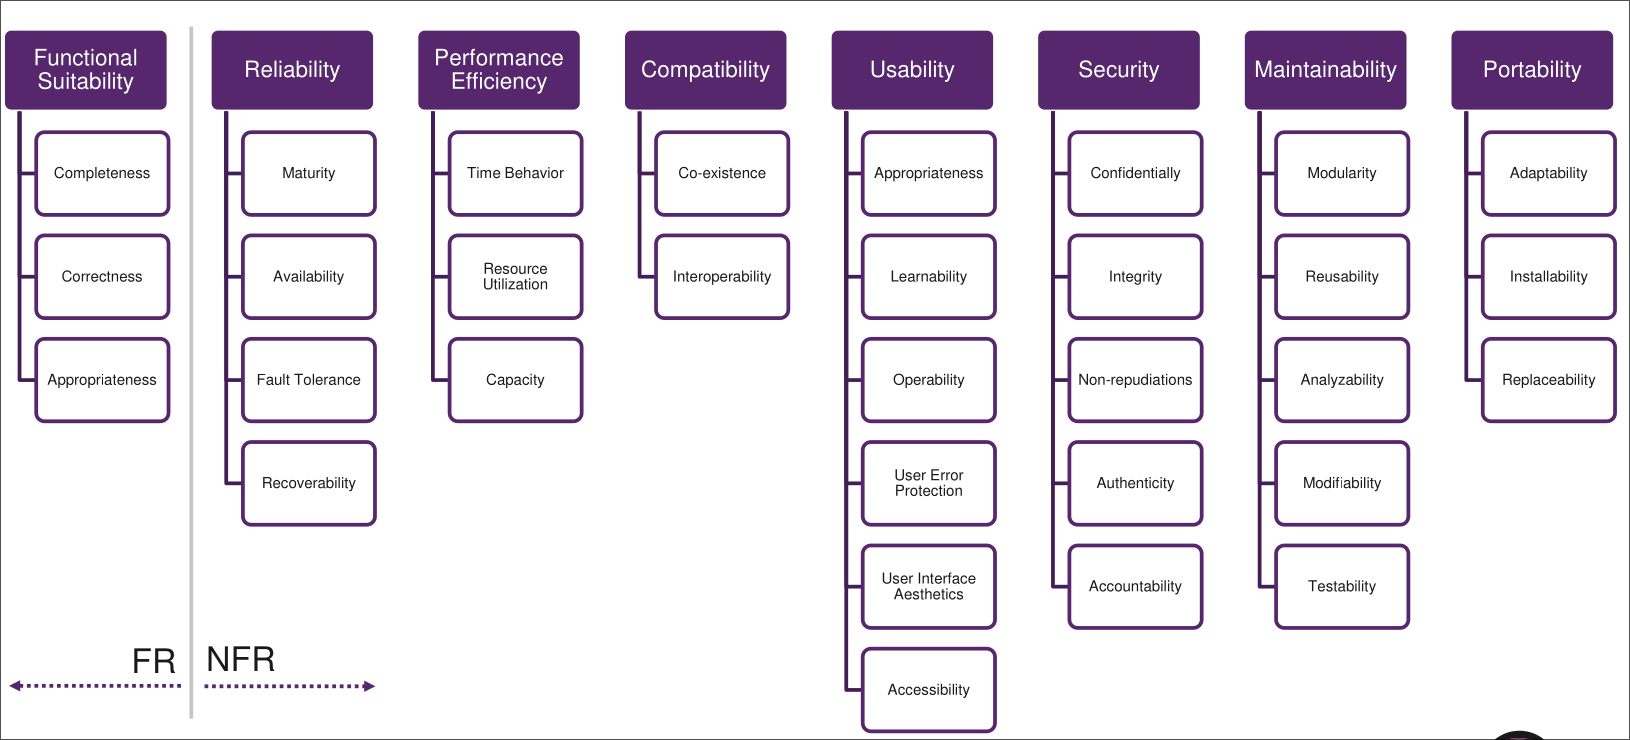
\includegraphics[scale=0.4]{2023_03_09_05_19_14.png}

\subsection{Overengineering and Underengineering}
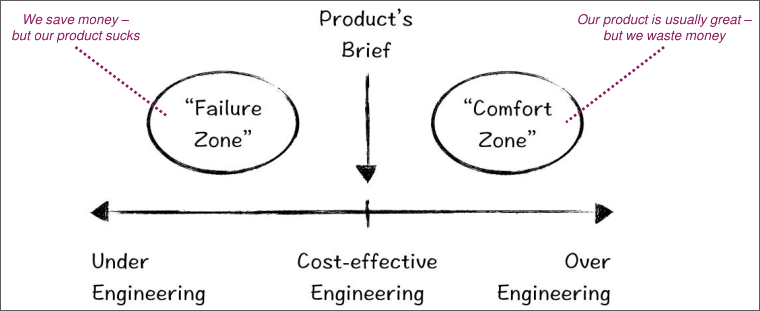
\includegraphics[scale=0.4]{2023_03_09_05_22_06.png}\newline
The right side wastes money, while the left side saves money at the cost of reputation.

\subsubsection{Technical Depth}
\textcolor{purple}{This is essentially just a backlog of things that you should still do. Ex. Tests, or better documentation, or a cleaner implementation.}\newline
Technical depth will often accumulate and you will end up at the left side, -> underengineering.\newline
It is important to keep track of this with developer stories and try to achieve \emph{more overengineering, rather than being complacent}.

\subsection{Software Aging}
\begin{itemize}
\item \textcolor{purple}{Causes}\newline
  \begin{itemize}
  \item \textcolor{black}{lack of change in technology}
  \item \textcolor{black}{update without thinking}
  \end{itemize} 
\item \textcolor{purple}{Costs}\newline
  \begin{itemize}
  \item \textcolor{black}{inability to keep up}
  \item \textcolor{black}{reduced performance}
  \item \textcolor{black}{decreasing reliability}
  \end{itemize} 
\item \textcolor{purple}{Remedy}\newline
  \begin{itemize}
  \item \textcolor{black}{stop the deterioration}
  \item \textcolor{black}{design for success}
  \item \textcolor{black}{plan ahead}
  \end{itemize} 
\end{itemize} 
\textcolor{red}{Important: Over time, the quality will pretty much always decline! -> wayland over Xorg!}

\subsubsection{Impact of complacency}
\textcolor{purple}{If you start to accept bugs, it will likely lead to more acceptence of more bugs. \newline
Eg. do not accept things such as not tested code, as it will likely reduce the quality of code in the long run!}

\subsubsection{Tools for Quality}
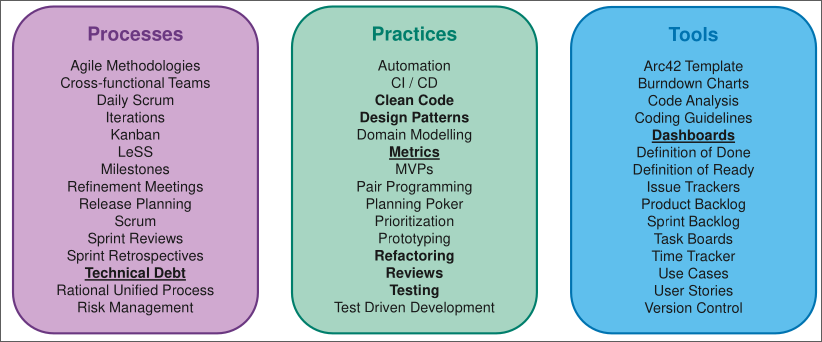
\includegraphics[scale=0.4]{2023_03_09_05_37_49.png}
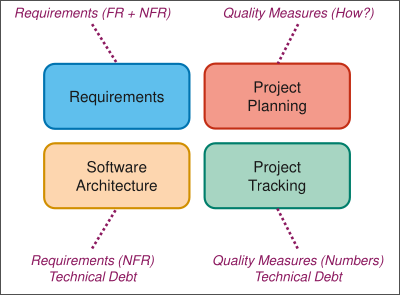
\includegraphics[scale=0.4]{2023_03_09_05_38_24.png}

\subsection{Maintainability of Code}
\begin{itemize}
\item \textcolor{purple}{POSIX function -> 1 functionality  per function}
\item \textcolor{purple}{Code Coverage}
\item \textcolor{purple}{Code Smells} LOC
\item \textcolor{purple}{Lines of code} CC
\item \textcolor{purple}{Cyclomatic Complexity} McCC
\end{itemize} 

\subsubsection{McCC}
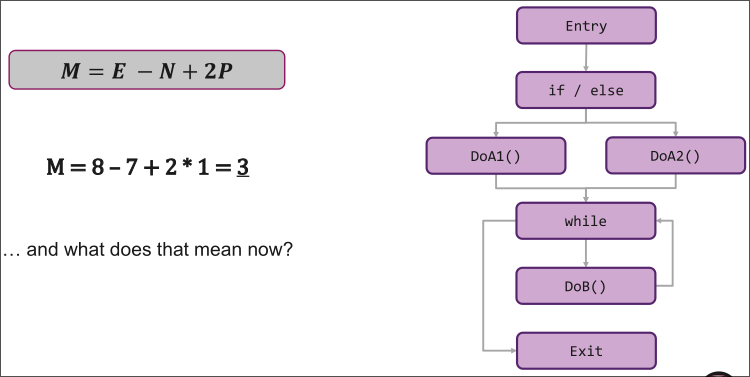
\includegraphics[scale=0.4]{2023_03_09_06_09_37.png}
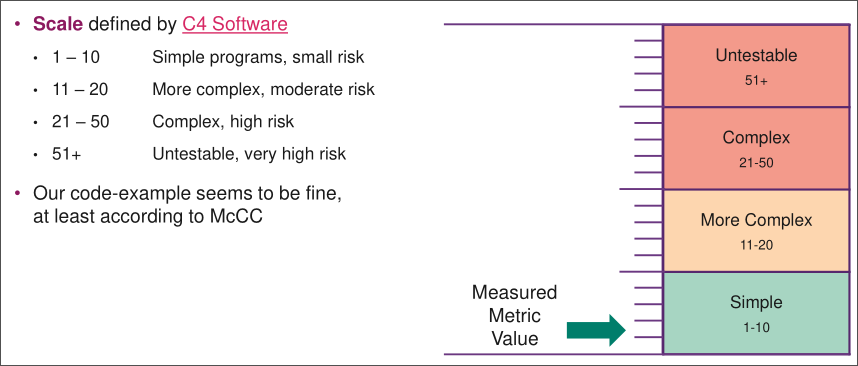
\includegraphics[scale=0.4]{2023_03_09_06_09_46.png}\newline
\textcolor{red}{Do NOT calculate this by hand, only let a tool do this task for you.}\newline
\textcolor{purple}{There are also a lot of tools that visualize the metric in order to stand out more to human eyes.}\newline
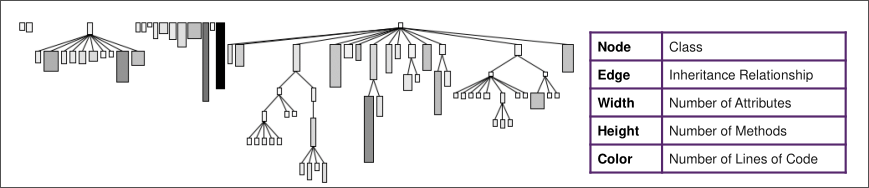
\includegraphics[scale=0.4]{2023_03_09_06_19_01.png}

\section{Software Architecture}
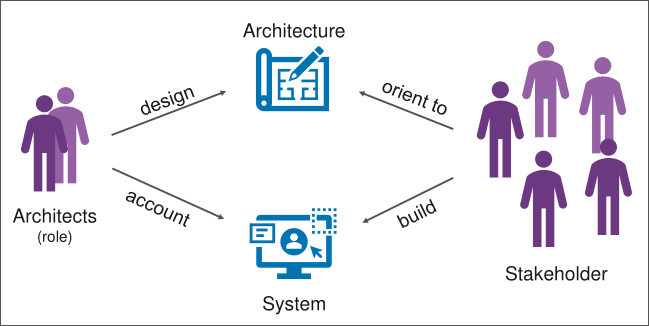
\includegraphics[scale=0.4]{2023_03_16_05_06_11.png}

\subsection{Architecture vs Design}
Architecture focuses on big changes while design is something that deals with smaller, more precise changes.

\subsection{Non-Functional Requirements}
\begin{itemize}
\item \textcolor{purple}{security}
\item \textcolor{purple}{reliability}
\item \textcolor{purple}{performance}
\item \textcolor{purple}{maintainability}
\item \textcolor{purple}{scalability}
\item \textcolor{purple}{usability}
\end{itemize} 
\textcolor{red}{These are often more important than the functional requirements, as it defines whether or not you can maintain this or not.\newline
Customers will often not like this, since it seems like a waste of time and money to them, but without this no software can truly become good.}

\subsection{Context and Components}
\textcolor{purple}{Drawing lines outside the system}\newline
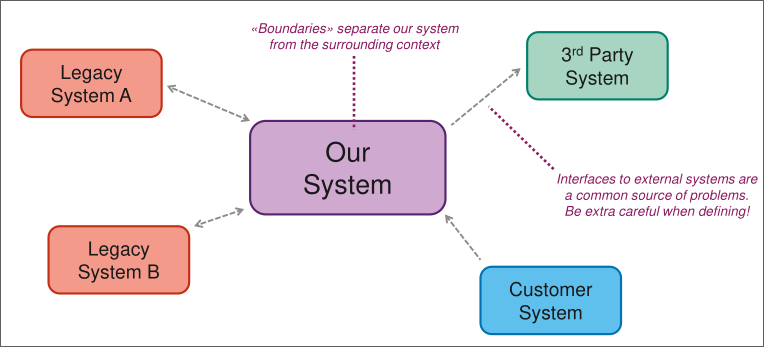
\includegraphics[scale=0.4]{2023_03_16_05_26_27.png}\newline
\textcolor{purple}{Drawing lines inside the system}\newline
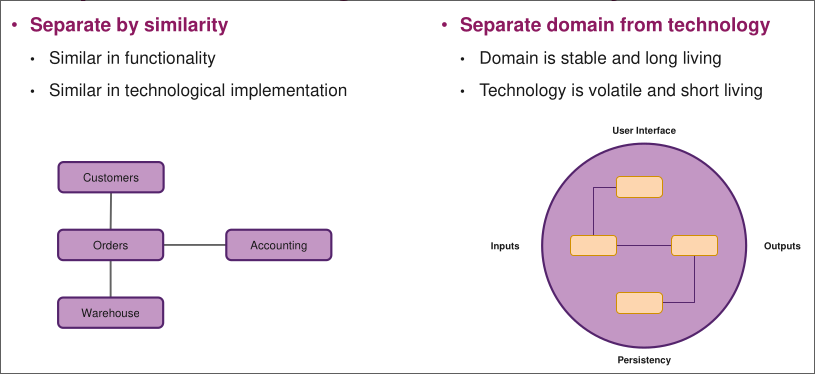
\includegraphics[scale=0.4]{2023_03_16_05_27_26.png}\newline
The idea here is that you need to make sure that you differentiate the domain model from the technology used.\newline
E.g you do not want to be dependent on jafuck with your software, it should also be possible to be written in a proper language such as rust.

\subsction{ACT Desirable Characteristics}
\begin{itemize}
\item \textcolor{purple}{Adequacy}
  Use proper tools for the job\newline
  Use as much time as needed... \newline
\item \textcolor{purple}{Timeliness}\newline
  Eliminate risks early\newline
  However, also leave some decicions out if possible -> iterative 
\item \textcolor{purple}{Consistency}\newline
\end{itemize} 

\subsection{The Software Architect Role}

\subsubsection{Responsibilities}
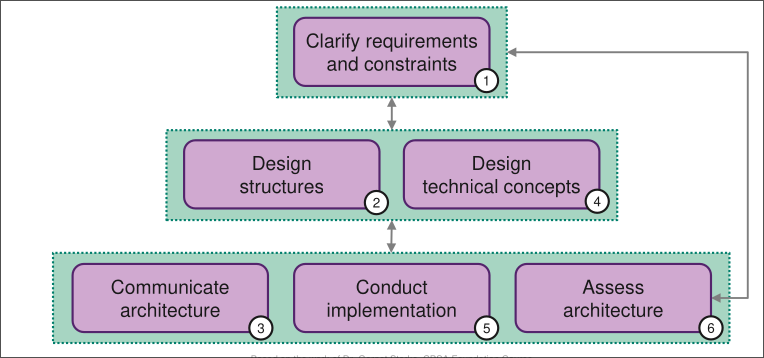
\includegraphics[scale=0.4]{2023_03_16_05_36_00.png}

\subsubsection{Different Types}
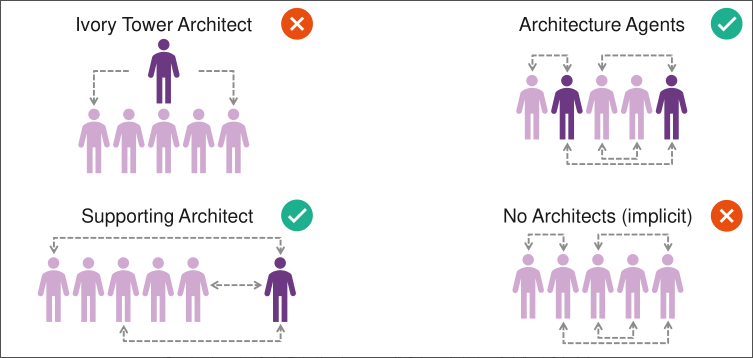
\includegraphics[scale=0.4]{2023_03_16_05_36_46.png}

\subsubsection{Scaling of the Role}
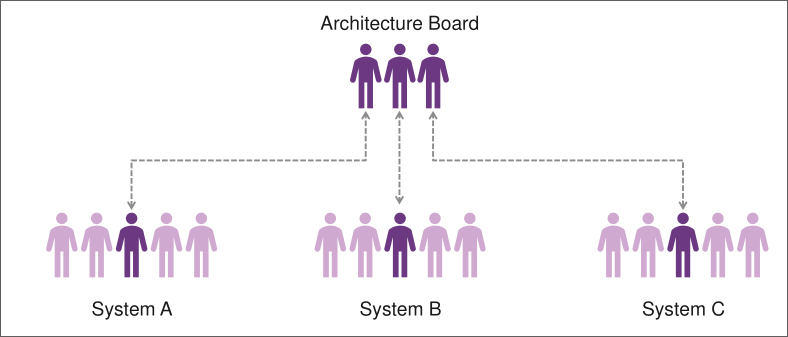
\includegraphics[scale=0.4]{2023_03_16_05_37_10.png}

\subsubsection{Communication of Architects}
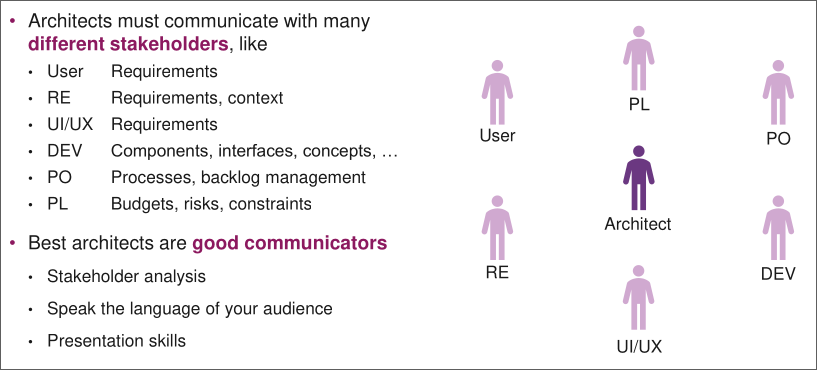
\includegraphics[scale=0.4]{2023_03_16_05_41_47.png}

\subsection{Documentation}
There are multiple templates that you can use in order to write your documentation. \newline
It is recommended that you use these templates as it makes your documentation more consistent.\newline
\begin{itemize}
\item \textcolor{purple}{arc42}
\item \textcolor{purple}{C4 model}
\item \textcolor{purple}{4+1 View Model of Architecture}
\item \textcolor{purple}{Software Architecture Document (SAD)}
\end{itemize} 
\textcolor{teal}{Most of them are \emph{high level}, and use \emph{building blocks}, with \emph{different views}.}

\subsubsection{arc42 Template}
\includegraphics[scale=0.4]{2023_03_16_06_24_43.png}

\subsection{Architectural Patterns}
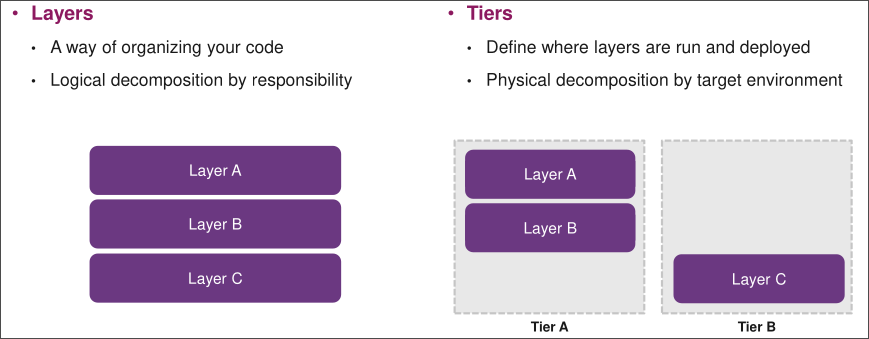
\includegraphics[scale=0.4]{2023_03_16_06_33_19.png}

\subsection{Architecture types}
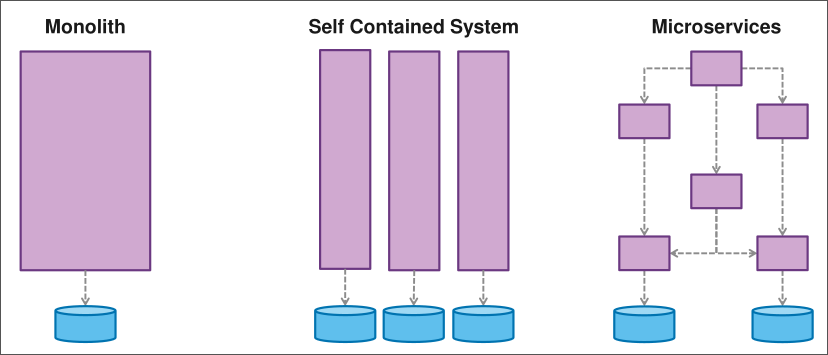
\includegraphics[scale=0.4]{2023_03_16_06_33_28.png}
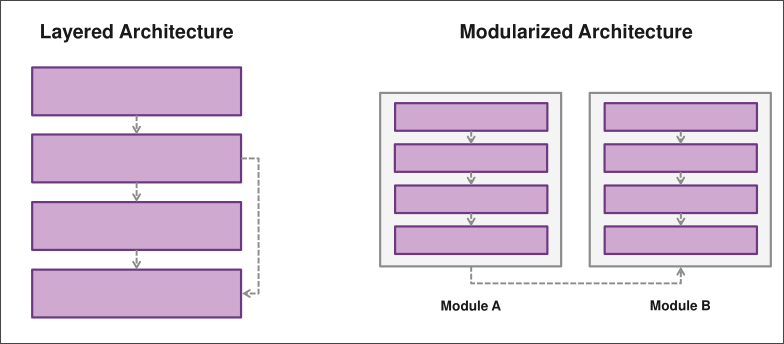
\includegraphics[scale=0.4]{2023_03_16_06_33_39.png}\newline
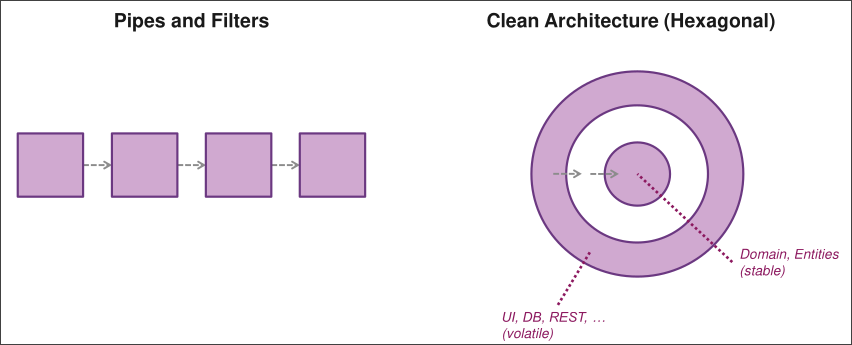
\includegraphics[scale=0.4]{2023_03_16_06_33_54.png}

\section{Software Craftmanship}

\subsection{The agile hangover}
\textcolor{teal}{There is one big problem with agile, it needs people that can work with it.\newline
It offers you more freedom, but requires that you actually value what you do. Meaning that you hold values such as clean code, proper architecture etc.}
Make note, it is not the goal to be perfect, but to simply hold and presue the value itself.

\subsection{Steps to be pragmatic}
\begin{enumerate}
\item \textcolor{purple}{Care about your craft}
\item \textcolor{purple}{Think about your work}
\item \textcolor{purple}{Provide options, don't make excuses}
\item \textcolor{purple}{Don't live with broken windows}
\item \textcolor{purple}{Be a catalyst for change}
\item \textcolor{purple}{Invest regularly in your knowledge portfolio}
\item \textcolor{purple}{Critically analyze what you read and hear}
\item \textcolor{purple}{Don't assume it, prove it}
\item \textcolor{purple}{Sign your work}
\item \textcolor{purple}{First, do no harm}

\end{enumerate} 



\includepdf[pages=-,scale=1]{../sep2/sep2-typst.pdf}

\end{document}

